\documentclass[twoside]{book}

% Packages required by doxygen
\usepackage{fixltx2e}
\usepackage{calc}
\usepackage{doxygen}
\usepackage[export]{adjustbox} % also loads graphicx
\usepackage{graphicx}
\usepackage[utf8]{inputenc}
\usepackage{makeidx}
\usepackage{multicol}
\usepackage{multirow}
\PassOptionsToPackage{warn}{textcomp}
\usepackage{textcomp}
\usepackage[nointegrals]{wasysym}
\usepackage[table]{xcolor}

% Font selection
\usepackage[T1]{fontenc}
\usepackage[scaled=.90]{helvet}
\usepackage{courier}
\usepackage{amssymb}
\usepackage{sectsty}
\renewcommand{\familydefault}{\sfdefault}
\allsectionsfont{%
  \fontseries{bc}\selectfont%
  \color{darkgray}%
}
\renewcommand{\DoxyLabelFont}{%
  \fontseries{bc}\selectfont%
  \color{darkgray}%
}
\newcommand{\+}{\discretionary{\mbox{\scriptsize$\hookleftarrow$}}{}{}}

% Page & text layout
\usepackage{geometry}
\geometry{%
  a4paper,%
  top=2.5cm,%
  bottom=2.5cm,%
  left=2.5cm,%
  right=2.5cm%
}
\tolerance=750
\hfuzz=15pt
\hbadness=750
\setlength{\emergencystretch}{15pt}
\setlength{\parindent}{0cm}
\setlength{\parskip}{3ex plus 2ex minus 2ex}
\makeatletter
\renewcommand{\paragraph}{%
  \@startsection{paragraph}{4}{0ex}{-1.0ex}{1.0ex}{%
    \normalfont\normalsize\bfseries\SS@parafont%
  }%
}
\renewcommand{\subparagraph}{%
  \@startsection{subparagraph}{5}{0ex}{-1.0ex}{1.0ex}{%
    \normalfont\normalsize\bfseries\SS@subparafont%
  }%
}
\makeatother

% Headers & footers
\usepackage{fancyhdr}
\pagestyle{fancyplain}
\fancyhead[LE]{\fancyplain{}{\bfseries\thepage}}
\fancyhead[CE]{\fancyplain{}{}}
\fancyhead[RE]{\fancyplain{}{\bfseries\leftmark}}
\fancyhead[LO]{\fancyplain{}{\bfseries\rightmark}}
\fancyhead[CO]{\fancyplain{}{}}
\fancyhead[RO]{\fancyplain{}{\bfseries\thepage}}
\fancyfoot[LE]{\fancyplain{}{}}
\fancyfoot[CE]{\fancyplain{}{}}
\fancyfoot[RE]{\fancyplain{}{\bfseries\scriptsize Generated by Doxygen }}
\fancyfoot[LO]{\fancyplain{}{\bfseries\scriptsize Generated by Doxygen }}
\fancyfoot[CO]{\fancyplain{}{}}
\fancyfoot[RO]{\fancyplain{}{}}
\renewcommand{\footrulewidth}{0.4pt}
\renewcommand{\chaptermark}[1]{%
  \markboth{#1}{}%
}
\renewcommand{\sectionmark}[1]{%
  \markright{\thesection\ #1}%
}

% Indices & bibliography
\usepackage{natbib}
\usepackage[titles]{tocloft}
\setcounter{tocdepth}{3}
\setcounter{secnumdepth}{5}
\makeindex

% Custom commands
\newcommand{\clearemptydoublepage}{%
  \newpage{\pagestyle{empty}\cleardoublepage}%
}

\usepackage{caption}
\captionsetup{labelsep=space,justification=centering,font={bf},singlelinecheck=off,skip=4pt,position=top}

%===== C O N T E N T S =====

\begin{document}

% Titlepage & ToC
\pagenumbering{alph}
\begin{titlepage}
\vspace*{7cm}
\begin{center}%
{\Large My Project }\\
\vspace*{1cm}
{\large Generated by Doxygen 1.8.14}\\
\end{center}
\end{titlepage}
\clearemptydoublepage
\pagenumbering{roman}
\tableofcontents
\clearemptydoublepage
\pagenumbering{arabic}

%--- Begin generated contents ---
\chapter{Namespace Index}
\section{Packages}
Here are the packages with brief descriptions (if available)\+:\begin{DoxyCompactList}
\item\contentsline{section}{\textbf{ model} }{\pageref{namespacemodel}}{}
\end{DoxyCompactList}

\chapter{Hierarchical Index}
\section{Class Hierarchy}
This inheritance list is sorted roughly, but not completely, alphabetically\+:\begin{DoxyCompactList}
\item \contentsline{section}{main.\+Goal\+Tracker}{\pageref{classmain_1_1_goal_tracker}}{}
\item \contentsline{section}{main.\+Goal\+Tracker\+Test}{\pageref{classmain_1_1_goal_tracker_test}}{}
\item \contentsline{section}{main.\+Goal\+Tracker\+Week}{\pageref{classmain_1_1_goal_tracker_week}}{}
\item \contentsline{section}{main.\+Task\+Viewer}{\pageref{classmain_1_1_task_viewer}}{}
\item Action\+Listener\begin{DoxyCompactList}
\item \contentsline{section}{main.\+Goal\+UI}{\pageref{classmain_1_1_goal_u_i}}{}
\item \contentsline{section}{main.\+Task\+UI}{\pageref{classmain_1_1_task_u_i}}{}
\end{DoxyCompactList}
\end{DoxyCompactList}

\chapter{Class Index}
\section{Class List}
Here are the classes, structs, unions and interfaces with brief descriptions\+:\begin{DoxyCompactList}
\item\contentsline{section}{\textbf{ model.\+Goal} }{\pageref{classmodel_1_1_goal}}{}
\item\contentsline{section}{\textbf{ model.\+Task} }{\pageref{classmodel_1_1_task}}{}
\item\contentsline{section}{\textbf{ model.\+Task\+Test} }{\pageref{classmodel_1_1_task_test}}{}
\end{DoxyCompactList}

\chapter{File Index}
\section{File List}
Here is a list of all files with brief descriptions\+:\begin{DoxyCompactList}
\item\contentsline{section}{\textbf{ Goal\+Tracker.\+java} }{\pageref{_goal_tracker_8java}}{}
\item\contentsline{section}{\textbf{ Goal\+Tracker\+Test.\+java} }{\pageref{_goal_tracker_test_8java}}{}
\item\contentsline{section}{\textbf{ Goal\+Tracker\+Week.\+java} }{\pageref{_goal_tracker_week_8java}}{}
\item\contentsline{section}{\textbf{ Goal\+U\+I.\+java} }{\pageref{_goal_u_i_8java}}{}
\item\contentsline{section}{\textbf{ Task\+U\+I.\+java} }{\pageref{_task_u_i_8java}}{}
\item\contentsline{section}{\textbf{ Task\+Viewer.\+java} }{\pageref{_task_viewer_8java}}{}
\end{DoxyCompactList}

\chapter{Namespace Documentation}
\section{Package main}
\label{namespacemain}\index{main@{main}}
\subsection*{Classes}
\begin{DoxyCompactItemize}
\item 
class \textbf{ Goal\+Tracker}
\item 
class \textbf{ Goal\+Tracker\+Test}
\item 
class \textbf{ Goal\+Tracker\+Week}
\item 
class \textbf{ Goal\+UI}
\item 
class \textbf{ Task\+UI}
\end{DoxyCompactItemize}

\chapter{Class Documentation}
\section{main.\+Goal\+Tracker Class Reference}
\label{classmain_1_1_goal_tracker}\index{main.\+Goal\+Tracker@{main.\+Goal\+Tracker}}
\subsection*{Classes}
\begin{DoxyCompactItemize}
\item 
class {\bfseries btn\+Next\+\_\+\+Action}
\item 
class {\bfseries btn\+Prev\+\_\+\+Action}
\item 
class {\bfseries cmb\+Year\+\_\+\+Action}
\item 
class {\bfseries tbl\+Calendar\+Renderer}
\end{DoxyCompactItemize}
\subsection*{Static Public Member Functions}
\begin{DoxyCompactItemize}
\item 
static void \textbf{ main} (String args[$\,$])
\item 
static void \textbf{ refresh\+Calendar} (int month, int year)
\end{DoxyCompactItemize}


\subsection{Member Function Documentation}
\mbox{\label{classmain_1_1_goal_tracker_a2039c98750da8b2c3136ff42d2682307}} 
\index{main\+::\+Goal\+Tracker@{main\+::\+Goal\+Tracker}!main@{main}}
\index{main@{main}!main\+::\+Goal\+Tracker@{main\+::\+Goal\+Tracker}}
\subsubsection{main()}
{\footnotesize\ttfamily static void main.\+Goal\+Tracker.\+main (\begin{DoxyParamCaption}\item[{String}]{args[$\,$] }\end{DoxyParamCaption})\hspace{0.3cm}{\ttfamily [static]}}

Calendar G\+UI. 
\begin{DoxyParams}{Parameters}
{\em args} & \\
\hline
\end{DoxyParams}
\mbox{\label{classmain_1_1_goal_tracker_a8257e39078e30681f0cc19ebc86d2041}} 
\index{main\+::\+Goal\+Tracker@{main\+::\+Goal\+Tracker}!refresh\+Calendar@{refresh\+Calendar}}
\index{refresh\+Calendar@{refresh\+Calendar}!main\+::\+Goal\+Tracker@{main\+::\+Goal\+Tracker}}
\subsubsection{refresh\+Calendar()}
{\footnotesize\ttfamily static void main.\+Goal\+Tracker.\+refresh\+Calendar (\begin{DoxyParamCaption}\item[{int}]{month,  }\item[{int}]{year }\end{DoxyParamCaption})\hspace{0.3cm}{\ttfamily [static]}}

Sets up the calendar. 
\begin{DoxyParams}{Parameters}
{\em month} & an int. \\
\hline
{\em year} & an int. \\
\hline
\end{DoxyParams}


The documentation for this class was generated from the following file\+:\begin{DoxyCompactItemize}
\item 
\textbf{ Goal\+Tracker.\+java}\end{DoxyCompactItemize}

\section{main.\+Goal\+Tracker\+Test Class Reference}
\label{classmain_1_1_goal_tracker_test}\index{main.\+Goal\+Tracker\+Test@{main.\+Goal\+Tracker\+Test}}


The documentation for this class was generated from the following file\+:\begin{DoxyCompactItemize}
\item 
\textbf{ Goal\+Tracker\+Test.\+java}\end{DoxyCompactItemize}

\section{main.\+Goal\+Tracker\+Week Class Reference}
\label{classmain_1_1_goal_tracker_week}\index{main.\+Goal\+Tracker\+Week@{main.\+Goal\+Tracker\+Week}}
\subsection*{Classes}
\begin{DoxyCompactItemize}
\item 
class {\bfseries btn\+Next\+\_\+\+Action}
\item 
class {\bfseries btn\+Prev\+\_\+\+Action}
\item 
class {\bfseries cmb\+Year\+\_\+\+Action}
\item 
class {\bfseries tbl\+Calendar\+Renderer}
\end{DoxyCompactItemize}
\subsection*{Static Public Member Functions}
\begin{DoxyCompactItemize}
\item 
static void \textbf{ main} (String args[$\,$])
\item 
static void \textbf{ refresh\+Calendar} (int week, int month, int year)
\end{DoxyCompactItemize}


\subsection{Member Function Documentation}
\mbox{\label{classmain_1_1_goal_tracker_week_a03418a3f1ae0a64e023b764cdba2fedb}} 
\index{main\+::\+Goal\+Tracker\+Week@{main\+::\+Goal\+Tracker\+Week}!main@{main}}
\index{main@{main}!main\+::\+Goal\+Tracker\+Week@{main\+::\+Goal\+Tracker\+Week}}
\subsubsection{main()}
{\footnotesize\ttfamily static void main.\+Goal\+Tracker\+Week.\+main (\begin{DoxyParamCaption}\item[{String}]{args[$\,$] }\end{DoxyParamCaption})\hspace{0.3cm}{\ttfamily [static]}}

\mbox{\label{classmain_1_1_goal_tracker_week_a7508790a7e52f9446de6160ad44bb938}} 
\index{main\+::\+Goal\+Tracker\+Week@{main\+::\+Goal\+Tracker\+Week}!refresh\+Calendar@{refresh\+Calendar}}
\index{refresh\+Calendar@{refresh\+Calendar}!main\+::\+Goal\+Tracker\+Week@{main\+::\+Goal\+Tracker\+Week}}
\subsubsection{refresh\+Calendar()}
{\footnotesize\ttfamily static void main.\+Goal\+Tracker\+Week.\+refresh\+Calendar (\begin{DoxyParamCaption}\item[{int}]{week,  }\item[{int}]{month,  }\item[{int}]{year }\end{DoxyParamCaption})\hspace{0.3cm}{\ttfamily [static]}}



The documentation for this class was generated from the following file\+:\begin{DoxyCompactItemize}
\item 
\textbf{ Goal\+Tracker\+Week.\+java}\end{DoxyCompactItemize}

\section{main.\+Goal\+UI Class Reference}
\label{classmain_1_1_goal_u_i}\index{main.\+Goal\+UI@{main.\+Goal\+UI}}


Inherits Action\+Listener.

\subsection*{Public Member Functions}
\begin{DoxyCompactItemize}
\item 
void \textbf{ action\+Performed} (Action\+Event e)
\end{DoxyCompactItemize}


\subsection{Member Function Documentation}
\mbox{\label{classmain_1_1_goal_u_i_a954aee8336c265d1f5058f1360261e14}} 
\index{main\+::\+Goal\+UI@{main\+::\+Goal\+UI}!action\+Performed@{action\+Performed}}
\index{action\+Performed@{action\+Performed}!main\+::\+Goal\+UI@{main\+::\+Goal\+UI}}
\subsubsection{action\+Performed()}
{\footnotesize\ttfamily void main.\+Goal\+U\+I.\+action\+Performed (\begin{DoxyParamCaption}\item[{Action\+Event}]{e }\end{DoxyParamCaption})}

Goal screen G\+UI. Closes the goal screen.

Saves the goal into the .csv file.

The documentation for this class was generated from the following file\+:\begin{DoxyCompactItemize}
\item 
\textbf{ Goal\+U\+I.\+java}\end{DoxyCompactItemize}

\section{main.\+Task\+UI Class Reference}
\label{classmain_1_1_task_u_i}\index{main.\+Task\+UI@{main.\+Task\+UI}}
Inheritance diagram for main.\+Task\+UI\+:\begin{figure}[H]
\begin{center}
\leavevmode
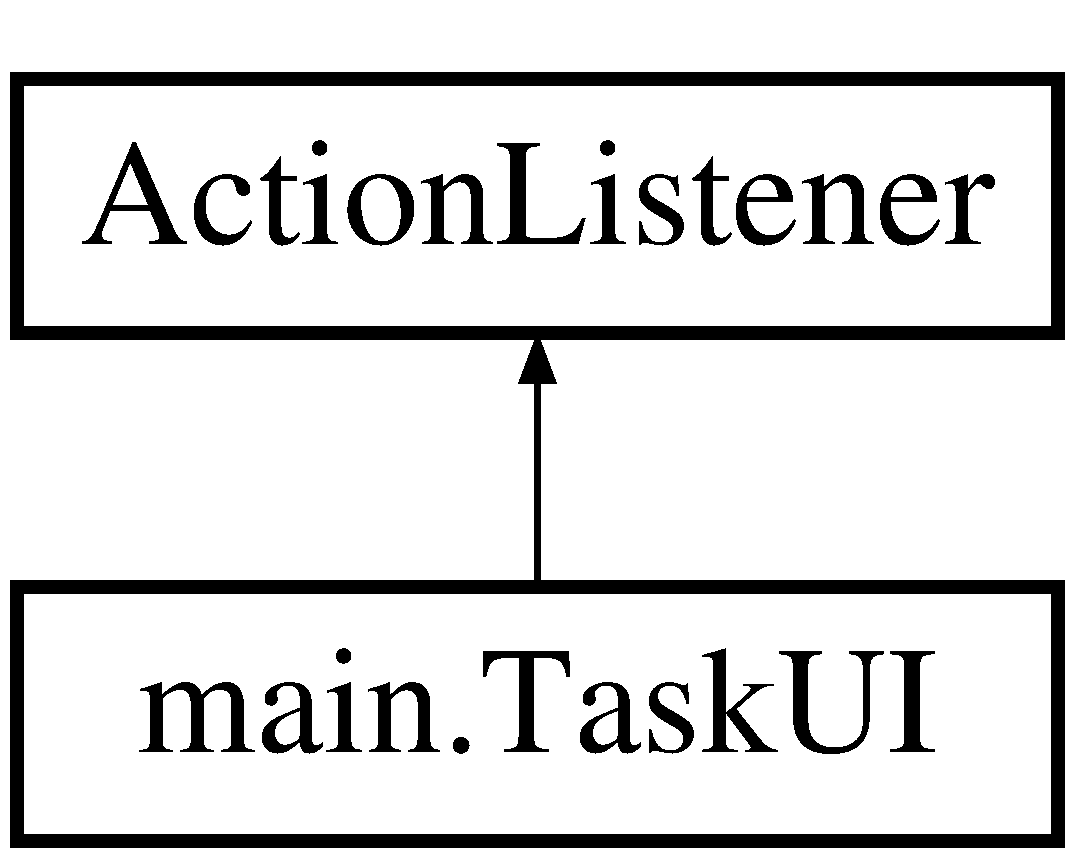
\includegraphics[height=2.000000cm]{classmain_1_1_task_u_i}
\end{center}
\end{figure}
\subsection*{Public Member Functions}
\begin{DoxyCompactItemize}
\item 
void \textbf{ action\+Performed} (Action\+Event e)
\item 
int \textbf{ get\+I\+D\+Count} ()
\item 
void \textbf{ add\+Tasks} (String titl, String desc, int s\+Month, int s\+Day, int s\+Year, int e\+Month, int e\+Day, int e\+Year, boolean urg, boolean imp, int id, int fT, String goal\+Desc, int g\+ID)
\item 
int \textbf{ convert\+Date} (int Month, int Day, int Year)
\item 
void \textbf{ create\+Tasks} (Task task)
\item 
void \textbf{ delete\+Tasks} (Task task)
\item 
void \textbf{ update\+Task} (Task old\+Task, Task new\+Task)
\item 
void \textbf{ fill\+List} (int day, int month, int year)
\end{DoxyCompactItemize}
\subsection*{Private Attributes}
\begin{DoxyCompactItemize}
\item 
Array\+List$<$ Task $>$ \textbf{ all\+Tasks} = new Array\+List$<$Task$>$()
\item 
int \textbf{ id\+Count}
\end{DoxyCompactItemize}


\subsection{Member Function Documentation}
\mbox{\label{classmain_1_1_task_u_i_ab9681721a6fd3d4cb8169c5633fed8c4}} 
\index{main\+::\+Task\+UI@{main\+::\+Task\+UI}!action\+Performed@{action\+Performed}}
\index{action\+Performed@{action\+Performed}!main\+::\+Task\+UI@{main\+::\+Task\+UI}}
\subsubsection{action\+Performed()}
{\footnotesize\ttfamily void main.\+Task\+U\+I.\+action\+Performed (\begin{DoxyParamCaption}\item[{Action\+Event}]{e }\end{DoxyParamCaption})}

Closes task screen.

Saves entered data into all\+Tasks Array\+List and into csv file.

Deletes all instances of the displayed task.\mbox{\label{classmain_1_1_task_u_i_aed31d359cf708f65c0e9fe646fb0a6e3}} 
\index{main\+::\+Task\+UI@{main\+::\+Task\+UI}!add\+Tasks@{add\+Tasks}}
\index{add\+Tasks@{add\+Tasks}!main\+::\+Task\+UI@{main\+::\+Task\+UI}}
\subsubsection{add\+Tasks()}
{\footnotesize\ttfamily void main.\+Task\+U\+I.\+add\+Tasks (\begin{DoxyParamCaption}\item[{String}]{titl,  }\item[{String}]{desc,  }\item[{int}]{s\+Month,  }\item[{int}]{s\+Day,  }\item[{int}]{s\+Year,  }\item[{int}]{e\+Month,  }\item[{int}]{e\+Day,  }\item[{int}]{e\+Year,  }\item[{boolean}]{urg,  }\item[{boolean}]{imp,  }\item[{int}]{id,  }\item[{int}]{fT,  }\item[{String}]{goal\+Desc,  }\item[{int}]{g\+ID }\end{DoxyParamCaption})}

Converts the info from start and end dates and creates tasks.


\begin{DoxyParams}{Parameters}
{\em titl} & a String title. \\
\hline
{\em desc} & a String description. \\
\hline
{\em s\+Month} & an int starting month. \\
\hline
{\em s\+Day} & an int starting day. \\
\hline
{\em s\+Year} & an int starting year. \\
\hline
{\em e\+Month} & an int ending month. \\
\hline
{\em e\+Day} & an int ending day. \\
\hline
{\em e\+Year} & and int ending year. \\
\hline
{\em urg} & a boolean urgency. \\
\hline
{\em imp} & a boolean importance. \\
\hline
{\em id} & and int task ID. \\
\hline
{\em fT} & and int task number. \\
\hline
{\em goal\+Desc} & a String description. \\
\hline
{\em g\+ID} & an int goal ID. \\
\hline
\end{DoxyParams}
\mbox{\label{classmain_1_1_task_u_i_a09dfe2f38b1807beeb29318e1ffafd62}} 
\index{main\+::\+Task\+UI@{main\+::\+Task\+UI}!convert\+Date@{convert\+Date}}
\index{convert\+Date@{convert\+Date}!main\+::\+Task\+UI@{main\+::\+Task\+UI}}
\subsubsection{convert\+Date()}
{\footnotesize\ttfamily int main.\+Task\+U\+I.\+convert\+Date (\begin{DoxyParamCaption}\item[{int}]{Month,  }\item[{int}]{Day,  }\item[{int}]{Year }\end{DoxyParamCaption})}

Converts the given month, day, and year into the day if the year 1-\/365.


\begin{DoxyParams}{Parameters}
{\em Month} & an int. \\
\hline
{\em Day} & an int. \\
\hline
{\em Year} & an int. \\
\hline
\end{DoxyParams}
\begin{DoxyReturn}{Returns}
an int day of year. 
\end{DoxyReturn}
\mbox{\label{classmain_1_1_task_u_i_aaac32305ea3fd0c6921db315f881c6a5}} 
\index{main\+::\+Task\+UI@{main\+::\+Task\+UI}!create\+Tasks@{create\+Tasks}}
\index{create\+Tasks@{create\+Tasks}!main\+::\+Task\+UI@{main\+::\+Task\+UI}}
\subsubsection{create\+Tasks()}
{\footnotesize\ttfamily void main.\+Task\+U\+I.\+create\+Tasks (\begin{DoxyParamCaption}\item[{Task}]{task }\end{DoxyParamCaption})}

Creates a task for each day the task is present.


\begin{DoxyParams}{Parameters}
{\em task} & a Task object. \\
\hline
\end{DoxyParams}
\mbox{\label{classmain_1_1_task_u_i_a6527ada9964eafbb2d283a14c96aeb4e}} 
\index{main\+::\+Task\+UI@{main\+::\+Task\+UI}!delete\+Tasks@{delete\+Tasks}}
\index{delete\+Tasks@{delete\+Tasks}!main\+::\+Task\+UI@{main\+::\+Task\+UI}}
\subsubsection{delete\+Tasks()}
{\footnotesize\ttfamily void main.\+Task\+U\+I.\+delete\+Tasks (\begin{DoxyParamCaption}\item[{Task}]{task }\end{DoxyParamCaption})}

Deletes all instances of a task.


\begin{DoxyParams}{Parameters}
{\em task} & a Task object. \\
\hline
\end{DoxyParams}
\mbox{\label{classmain_1_1_task_u_i_a1dfb5cce70e2c7ef333e4f4c99d6c029}} 
\index{main\+::\+Task\+UI@{main\+::\+Task\+UI}!fill\+List@{fill\+List}}
\index{fill\+List@{fill\+List}!main\+::\+Task\+UI@{main\+::\+Task\+UI}}
\subsubsection{fill\+List()}
{\footnotesize\ttfamily void main.\+Task\+U\+I.\+fill\+List (\begin{DoxyParamCaption}\item[{int}]{day,  }\item[{int}]{month,  }\item[{int}]{year }\end{DoxyParamCaption})}

Fills the day.\+csv file.


\begin{DoxyParams}{Parameters}
{\em day} & an int. \\
\hline
{\em month} & an int. \\
\hline
{\em year} & an int. \\
\hline
\end{DoxyParams}
\mbox{\label{classmain_1_1_task_u_i_a8bee5cf0d378c2e4f4b7b728407c4c4a}} 
\index{main\+::\+Task\+UI@{main\+::\+Task\+UI}!get\+I\+D\+Count@{get\+I\+D\+Count}}
\index{get\+I\+D\+Count@{get\+I\+D\+Count}!main\+::\+Task\+UI@{main\+::\+Task\+UI}}
\subsubsection{get\+I\+D\+Count()}
{\footnotesize\ttfamily int main.\+Task\+U\+I.\+get\+I\+D\+Count (\begin{DoxyParamCaption}{ }\end{DoxyParamCaption})}

Gets the generated unique task ID.

\begin{DoxyReturn}{Returns}
the int task ID. 
\end{DoxyReturn}
\mbox{\label{classmain_1_1_task_u_i_af2691e90b6fa38cea7176dc3c709c198}} 
\index{main\+::\+Task\+UI@{main\+::\+Task\+UI}!update\+Task@{update\+Task}}
\index{update\+Task@{update\+Task}!main\+::\+Task\+UI@{main\+::\+Task\+UI}}
\subsubsection{update\+Task()}
{\footnotesize\ttfamily void main.\+Task\+U\+I.\+update\+Task (\begin{DoxyParamCaption}\item[{Task}]{old\+Task,  }\item[{Task}]{new\+Task }\end{DoxyParamCaption})}



\subsection{Member Data Documentation}
\mbox{\label{classmain_1_1_task_u_i_a05bb12a52cb66bc7ef6b0a001108bd06}} 
\index{main\+::\+Task\+UI@{main\+::\+Task\+UI}!all\+Tasks@{all\+Tasks}}
\index{all\+Tasks@{all\+Tasks}!main\+::\+Task\+UI@{main\+::\+Task\+UI}}
\subsubsection{all\+Tasks}
{\footnotesize\ttfamily Array\+List$<$Task$>$ main.\+Task\+U\+I.\+all\+Tasks = new Array\+List$<$Task$>$()\hspace{0.3cm}{\ttfamily [private]}}

\mbox{\label{classmain_1_1_task_u_i_ac561a3128768f58d8c9ddeadc2edddf3}} 
\index{main\+::\+Task\+UI@{main\+::\+Task\+UI}!id\+Count@{id\+Count}}
\index{id\+Count@{id\+Count}!main\+::\+Task\+UI@{main\+::\+Task\+UI}}
\subsubsection{id\+Count}
{\footnotesize\ttfamily int main.\+Task\+U\+I.\+id\+Count\hspace{0.3cm}{\ttfamily [private]}}



The documentation for this class was generated from the following file\+:\begin{DoxyCompactItemize}
\item 
\textbf{ Task\+U\+I.\+java}\end{DoxyCompactItemize}

\chapter{File Documentation}
\section{Goal\+Tracker.\+java File Reference}
\label{_goal_tracker_8java}\index{Goal\+Tracker.\+java@{Goal\+Tracker.\+java}}
\subsection*{Classes}
\begin{DoxyCompactItemize}
\item 
class \textbf{ main.\+Goal\+Tracker}
\item 
class {\bfseries main.\+Goal\+Tracker.\+tbl\+Calendar\+Renderer}
\item 
class {\bfseries main.\+Goal\+Tracker.\+btn\+Prev\+\_\+\+Action}
\item 
class {\bfseries main.\+Goal\+Tracker.\+btn\+Next\+\_\+\+Action}
\item 
class {\bfseries main.\+Goal\+Tracker.\+cmb\+Year\+\_\+\+Action}
\item 
class {\bfseries main.\+Goal\+Tracker.\+btn\+Date\+\_\+\+Action}
\end{DoxyCompactItemize}
\subsection*{Packages}
\begin{DoxyCompactItemize}
\item 
package \textbf{ main}
\end{DoxyCompactItemize}

\section{Goal\+Tracker\+Test.\+java File Reference}
\label{_goal_tracker_test_8java}\index{Goal\+Tracker\+Test.\+java@{Goal\+Tracker\+Test.\+java}}
\subsection*{Classes}
\begin{DoxyCompactItemize}
\item 
class \textbf{ main.\+Goal\+Tracker\+Test}
\end{DoxyCompactItemize}
\subsection*{Packages}
\begin{DoxyCompactItemize}
\item 
package \textbf{ main}
\end{DoxyCompactItemize}

\section{Goal\+Tracker\+Week.\+java File Reference}
\label{_goal_tracker_week_8java}\index{Goal\+Tracker\+Week.\+java@{Goal\+Tracker\+Week.\+java}}
\subsection*{Classes}
\begin{DoxyCompactItemize}
\item 
class \textbf{ main.\+Goal\+Tracker\+Week}
\item 
class {\bfseries main.\+Goal\+Tracker\+Week.\+tbl\+Calendar\+Renderer}
\item 
class {\bfseries main.\+Goal\+Tracker\+Week.\+btn\+Prev\+\_\+\+Action}
\item 
class {\bfseries main.\+Goal\+Tracker\+Week.\+btn\+Next\+\_\+\+Action}
\item 
class {\bfseries main.\+Goal\+Tracker\+Week.\+cmb\+Year\+\_\+\+Action}
\end{DoxyCompactItemize}
\subsection*{Packages}
\begin{DoxyCompactItemize}
\item 
package \textbf{ main}
\end{DoxyCompactItemize}

\section{Goal\+U\+I.\+java File Reference}
\label{_goal_u_i_8java}\index{Goal\+U\+I.\+java@{Goal\+U\+I.\+java}}
\subsection*{Classes}
\begin{DoxyCompactItemize}
\item 
class \textbf{ main.\+Goal\+UI}
\end{DoxyCompactItemize}
\subsection*{Packages}
\begin{DoxyCompactItemize}
\item 
package \textbf{ main}
\end{DoxyCompactItemize}

\section{Task\+U\+I.\+java File Reference}
\label{_task_u_i_8java}\index{Task\+U\+I.\+java@{Task\+U\+I.\+java}}
\subsection*{Classes}
\begin{DoxyCompactItemize}
\item 
class \textbf{ main.\+Task\+UI}
\end{DoxyCompactItemize}
\subsection*{Packages}
\begin{DoxyCompactItemize}
\item 
package \textbf{ main}
\end{DoxyCompactItemize}

%--- End generated contents ---

% Index
\backmatter
\newpage
\phantomsection
\clearemptydoublepage
\addcontentsline{toc}{chapter}{Index}
\printindex

\end{document}
